\section{Medición y Error Experimental Con Frijoles}
\subsection{Objetivos}
\begin{itemize}
	\item Determinar la incertidumbre en el siguiente proceso de medición.
	\item Determinar la curva de distribución normal en un proceso de medición, correspondiente al numero de frijoles que caben en vaso seleccionado previamente.
\end{itemize}

\subsection{Fundamento teórico}
\begin{itemize}
	\item \textbf{Medición:} La medición es un proceso básico de la ciencia que se basa en comparar
	      una unidad de medida seleccionada con el objeto o fenómeno cuya magnitud física se
	      desea medir, para averiguar cuantas veces la unidad está contenida en esa magnitud.
	\item \textbf{Incertidumbre :} Es el parámetro asociado con el resultado de una medición, que
	      caracteriza la dispersión de los valores que podrían ser razonablemente atribuidos al
	      valor a medir. Por ejemplo: Un experimentador que haga la misma medición muchas
	      veces no obtendrá los mismos resultados tanto por factores externos como (luz, viento,
	      etc.) como las variaciones en las condiciones de observación del experimentador.
	\item \textbf{Ajuste de Curva: } El ajuste de curvas consiste en encontrar una curva que contenga
	      una serie de puntos y que posiblemente cumpla una serie de restricciones adicionales.
	      Esta sección es una introducción tanto a la interpolación (cuando se espera un ajuste
	      exacto a determinadas restricciones) y al ajuste de curvas/análisis de regresión (cuando
	      se permite una aproximación).
\end{itemize}
\subsection{Materiales y equipos de trabajo}

\begin{figure}[H]
	\begin{center}
		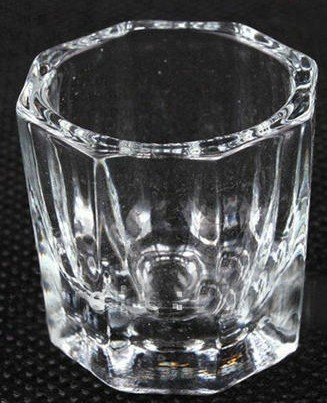
\includegraphics[width = 0.3\textwidth]{Imagenes/vaso.jpg}
		\captionof{figure}{\label{fig:vaso}vaso pequeño}
	\end{center}
\end{figure}
\begin{figure}[H]
	\begin{center}
		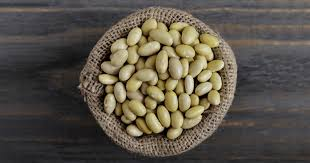
\includegraphics[width = 0.4\textwidth]{Imagenes/frijoles.jpeg}
		\captionof{figure}{\label{fig:frijoles}frijoles 250gr}
	\end{center}
\end{figure}

\subsection{Resultados y Procedimientos}



\subsubsection{Procedimientos}

\begin{enumerate}
	\item Colocar el vaso sobre una mesa
	\item Vaciar los frejoles en el vaso hasta que se llene. Que no rebase el tope o se aleje mucho de él.
	\item Contar el número de frejoles, devolverlo a la bolsa y sacudirla (Para de evitar sacar los mismos frijoles)
	\item Escribir los resultados en una tabla de (4x100), donde las columnas se encabezan por:
	      \begin{itemize}
		      \item $K$ : k- esimo conteo
		      \item $N_k$ : el K-esimo conteo de frijoles
		      \item $N_k - \overline{mnp}$ :  k-esimo conteo - el promedio
		      \item $(N_k - \overline{mnp})^2$ : k-esimo conteo - el promedio, al cuadrado
	      \end{itemize}
	\item Repetir hasta tener 100 repeticiones en total
	\item Determinar la media aritmética $\overline{mnp}$ de los 100 números obtenidos. Esta media aritmética es el número más probable de frijoles que caben en el vaso.

	      Sea $N_k$ el número de frijoles obtenidos en la k-ésima operación. La media aritmética de los 100 números obtenidos es:
	      \begin{equation*}
		      \overline{mnp}=\dfrac{1}{100}\sum_{i=1}^{100} N_k = 144.86
	      \end{equation*}
	\item Determine la incertidumbre normal o desviación estándar,$\Delta(\overline{mnp})$ , de la medición anterior.

	      La incertidumbre normal o desviación estándar será:
	      \begin{equation*}
		      \Delta(\overline{n m p})=\sqrt{\frac{1}{100} \sum_{k=1}^{100}\left(N_k-\overline{mnp}\right)^2}=4.622
	      \end{equation*}
	\item Grafique tanto la posibilidad $n(r,r+1)$ y $n(r,r+2)$

\end{enumerate}

\newpage
\subsubsection{Resultados}

\begin{xltabular}{\textwidth}{|c|c|c|c|}
	\caption{tabla de resultados de conteo} \\

	\hline \multicolumn{1}{|c|}{\textbf{K}} & \multicolumn{1}{c|}{\textbf{$N_k$}} & \multicolumn{1}{c|}{\textbf{$N_k - \overline{mnp} $}} & \multicolumn{1}{c|}{\textbf{$(N_k - \overline{mnp})^2$}} \\ \hline
	\endfirsthead

	\multicolumn{3}{c}%
	{} \\
	\hline
	\endhead

	\hline \multicolumn{4}{|r|}{{Continued on next page}} \\ \hline
	\endfoot

	\hline
	\endlastfoot

	1   & 145 & 0,14  & 0,02  \\
	2   & 144 & -0,86 & 0,74  \\
	3   & 154 & 9,14  & 83,54 \\
	4   & 145 & 0,14  & 0,02  \\
	5   & 150 & 5,14  & 26,42 \\
	6   & 139 & -5,86 & 34,34 \\
	7   & 143 & -1,86 & 3,46  \\
	8   & 140 & -4,86 & 23,62 \\
	9   & 143 & -1,86 & 3,46  \\
	10  & 144 & -0,86 & 0,74  \\
	11  & 146 & 1,14  & 1,30  \\
	12  & 152 & 7,14  & 50,98 \\
	13  & 148 & 3,14  & 9,86  \\
	14  & 144 & -0,86 & 0,74  \\
	15  & 151 & 6,14  & 37,70 \\
	16  & 150 & 5,14  & 26,42 \\
	17  & 148 & 3,14  & 9,86  \\
	18  & 152 & 7,14  & 50,98 \\
	19  & 149 & 4,14  & 17,14 \\
	20  & 145 & 0,14  & 0,02  \\
	21  & 143 & -1,86 & 3,46  \\
	22  & 144 & -0,86 & 0,74  \\
	23  & 146 & 1,14  & 1,30  \\
	24  & 143 & -1,86 & 3,46  \\
	25  & 142 & -2,86 & 8,18  \\
	26  & 144 & -0,86 & 0,74  \\
	27  & 143 & -1,86 & 3,46  \\
	28  & 147 & 2,14  & 4,58  \\
	29  & 150 & 5,14  & 26,42 \\
	30  & 149 & 4,14  & 17,14 \\
	31  & 152 & 7,14  & 50,98 \\
	32  & 146 & 1,14  & 1,30  \\
	33  & 151 & 6,14  & 37,70 \\
	34  & 141 & -3,86 & 14,90 \\
	35  & 148 & 3,14  & 9,86  \\
	36  & 148 & 3,14  & 9,86  \\
	37  & 146 & 1,14  & 1,30  \\
	38  & 150 & 5,14  & 26,42 \\
	39  & 146 & 1,14  & 1,30  \\
	40  & 149 & 4,14  & 17,14 \\
	41  & 146 & 1,14  & 1,30  \\
	42  & 148 & 3,14  & 9,86  \\
	43  & 147 & 2,14  & 4,58  \\
	44  & 153 & 8,14  & 66,26 \\
	45  & 145 & 0,14  & 0,02  \\
	46  & 147 & 2,14  & 4,58  \\
	47  & 147 & 2,14  & 4,58  \\
	48  & 142 & -2,86 & 8,18  \\
	49  & 154 & 9,14  & 83,54 \\
	50  & 143 & -1,86 & 3,46  \\
	51  & 146 & 1,14  & 1,30  \\
	52  & 145 & 0,14  & 0,02  \\
	53  & 147 & 2,14  & 4,58  \\
	54  & 137 & -7,86 & 61,78 \\
	55  & 144 & -0,86 & 0,74  \\
	56  & 143 & -1,86 & 3,46  \\
	57  & 145 & 0,14  & 0,02  \\
	58  & 138 & -6,86 & 47,06 \\
	59  & 136 & -8,86 & 78,50 \\
	60  & 142 & -2,86 & 8,18  \\
	61  & 141 & -3,86 & 14,90 \\
	62  & 138 & -6,86 & 47,06 \\
	63  & 153 & 8,14  & 66,26 \\
	64  & 145 & 0,14  & 0,02  \\
	65  & 148 & 3,14  & 9,86  \\
	66  & 145 & 0,14  & 0,02  \\
	67  & 146 & 1,14  & 1,30  \\
	68  & 144 & -0,86 & 0,74  \\
	69  & 142 & -2,86 & 8,18  \\
	70  & 140 & -4,86 & 23,62 \\
	71  & 141 & -3,86 & 14,90 \\
	72  & 140 & -4,86 & 23,62 \\
	73  & 145 & 0,14  & 0,02  \\
	74  & 139 & -5,86 & 34,34 \\
	75  & 145 & 0,14  & 0,02  \\
	76  & 147 & 2,14  & 4,58  \\
	77  & 146 & 1,14  & 1,30  \\
	78  & 149 & 4,14  & 17,14 \\
	79  & 139 & -5,86 & 34,34 \\
	80  & 147 & 2,14  & 4,58  \\
	81  & 144 & -0,86 & 0,74  \\
	82  & 146 & 1,14  & 1,30  \\
	83  & 150 & 5,14  & 26,42 \\
	84  & 152 & 7,14  & 50,98 \\
	85  & 140 & -4,86 & 23,62 \\
	86  & 151 & 6,14  & 37,70 \\
	87  & 147 & 2,14  & 4,58  \\
	88  & 141 & -3,86 & 14,90 \\
	89  & 137 & -7,86 & 61,78 \\
	90  & 144 & -0,86 & 0,74  \\
	91  & 140 & -4,86 & 23,62 \\
	92  & 139 & -5,86 & 34,34 \\
	93  & 138 & -6,86 & 47,06 \\
	94  & 142 & -2,86 & 8,18  \\
	95  & 141 & -3,86 & 14,90 \\
	96  & 138 & -6,86 & 47,06 \\
	97  & 141 & -3,86 & 14,90 \\
	98  & 145 & 0,14  & 0,02  \\
	99  & 138 & -6,86 & 47,06 \\
	100 & 137 & -7,86 & 61,78 \\
\end{xltabular}

\begin{xltabular}{\textwidth}{|c|c|c|}
	\caption{tabla de posibilidad de $n(r,r+1)$} \\

	\hline \multicolumn{1}{|c|}{\textbf{Número de frijoles}} & \multicolumn{1}{c|}{\textbf{$n(r,r+1)$}} & \multicolumn{1}{c|}{\textbf{$\pi(r,r+1)$}}  \\ \hline
	\endfirsthead

	\multicolumn{3}{c}%
	{} \\
	\hline
	\endhead

	\hline \multicolumn{3}{|r|}{{Continued on next page}} \\ \hline
	\endfoot

	\hline
	\endlastfoot
	136 & 1  & 0,01 \\
	137 & 3  & 0,03 \\
	138 & 5  & 0,05 \\
	139 & 4  & 0,04 \\
	140 & 5  & 0,05 \\
	141 & 6  & 0,06 \\
	142 & 5  & 0,05 \\
	143 & 7  & 0,07 \\
	144 & 9  & 0,09 \\
	145 & 11 & 0,11 \\
	146 & 10 & 0,1  \\
	147 & 8  & 0,08 \\
	148 & 6  & 0,06 \\
	149 & 4  & 0,04 \\
	150 & 5  & 0,05 \\
	151 & 3  & 0,03 \\
	152 & 4  & 0,04 \\
	153 & 2  & 0,02 \\
	154 & 2  & 0,02 \\ \hline
\end{xltabular}

\begin{xltabular}{\textwidth}{|c|c|c|}
	\caption{tabla de posibilidad de $n(r,r+2)$} \\

	\hline \multicolumn{1}{|c|}{\textbf{Número de frijoles}} & \multicolumn{1}{c|}{\textbf{$n(r,r+2)$}} & \multicolumn{1}{c|}{\textbf{$\pi(r,r+1)$}}  \\ \hline
	\endfirsthead

	\multicolumn{3}{c}%
	{} \\
	\hline
	\endhead

	\hline \multicolumn{3}{|r|}{{Continued on next page}} \\ \hline
	\endfoot

	\hline
	\endlastfoot
	136 - 138 & 4  & 0,04 \\
	138 - 140 & 9  & 0,09 \\
	140 - 142 & 11 & 0,11 \\
	142 - 144 & 12 & 0,12 \\
	144 - 146 & 20 & 0,2  \\
	146 - 148 & 18 & 0,18 \\
	148 - 150 & 10 & 0,1  \\
	150 - 152 & 8  & 0,08 \\
	152 - 154 & 6  & 0,06 \\
	154 - 156 & 2  & 0,02
\end{xltabular}

\subsection{Preguntas}
\begin{enumerate}
	\item  \textbf{En vez de medir puñados, ¿podría medirse el número de frijoles que caben en
		      un vaso, en una cuchara, etc.?}

	      Sería preferible medir con un vaso ya que el volumen que recogerá se mantendrá relativamente constante. Sobre diferencia entre los puñados se debe a la forma, tamaño y agarre de la mano de cada participante y de su criterio sobre lo que es flojo o apretado.
	      \item. \textbf{Después de realizar los experimentos, ¿qué ventaja le ve a la representación de $\pi [r, r+2)$ frente a la de $\pi [r, r+1)$?}

	      A pesar de que esta pierda precisión respecto a [r, r+1), sus resultados mostrados son más consistentes y fáciles de procesar.
	\item  \textbf{¿Qué sucedería si los frijoles fuesen de tamaños apreciablemente diferentes?}

	      Las mediciones variarían de forma considerable, incluso llegando a resultados drásticamente alejados de la media.
	\item \textbf{En el ejemplo mostrado se debía contar alrededor de 60 frijoles por puñado. ¿Sería ventajoso colocar solo 100 frijoles en el recipiente, y de esta manera calcular el número de frijoles en un puñado contando los frijoles que quedan en el recipiente?}

	      Respecto a la velocidad de medición sería ventajoso realizarlo de esa manera, sin embargo los resultados solo serían confiables respecto a un grupo muy reducido (de 100) en comparación con la muestra original (que sería mucho mayor), debido a que las distintas variaciones dentro de ese grupo podrían ser una representación incorrecta al momento de abarcar una muestra mayo
	\item \textbf{¿Qué sucedería si en el caso anterior colocara solo, digamos 75 frijoles en el
		      recipiente?}

	      La variación sería incluso menor que en la medición de 100 frijoles, y los casos donde se repitan los mismos grupos de frijoles serían más probables.
	\item \textbf{La parte de este experimento que exige ¨más paciencia¨ es el proceso de
		      contar. Para distribuir esta tarea entre tres personas. ¿Cuál de las sugerencias
		      propondría Ud.? ¿Por qué?}

	      Usar tres recipientes del mismo tamaño y forma, porque ahí el volumen es constante y la muestra recogida a solo se sujeta a las variaciones de tamaño de los frijoles y no del contenedor (la mano)
	\item \textbf{Mencione tres posibles hechos que observarían si en vez de 100 puñados
		      extrajeran 1000 puñados.}

	      \begin{enumerate}
		      \item  La variación estándar será diferente y más fiable
		      \item La gráfica de frecuencias se aproximaría más a la campana de gauss
		      \item Las mediciones podrían verse afectadas por la fatiga de los participantes si se mantiene el método actual de conteo (1 por 1)
	      \end{enumerate}
	\item \textbf{¿Cuál es el promedio aritmético de las desviaciones $Nk - \overline{mnp}$ ?}

	      El promedio es 0, debido a que hay variaciones positivas y negativas respecto al promedio y al sumarlas todas se anulan mutuamente.
	\item \textbf{¿Cuál cree Ud. es la razón para haber definido $\Delta \overline{mnp}$ en vez de tomar
		      simplemente el promedio de las desviaciones?}

	      La razón fue justamente evitar la anulación del resultado al convertir los valores negativos a positivos y obtener un resultado pertinente.
	\item \textbf{Después de realizar el experimento coja Ud. un puñado de frijoles. ¿Qué puede
		      Ud. afirmar sobre el número de frijoles contenido en tal puño (antes de contar)?}

	      Se puede afirmar que la cantidad a ser contada será cercana al promedio obtenido
	\item \textbf{Mencione Ud. alguna ventaja o desventaja de emplear pallares en vez de
		      frijoles en el presente experimento.}

	      Como ventaja sería más rápido el conteo, sin embargo por su mayor tamaño y forma irregular respecto a los frejoles crearía mayores espacios de vacío que afectarían a la medición
\end{enumerate}
